
\documentclass[11pt]{article}
\usepackage[a4paper,margin=0.75in]{geometry}
\usepackage{fontspec}
\usepackage{xeCJK}
\setmainfont{Helvetica Neue}
\setCJKmainfont{Songti TC}
\usepackage{booktabs}
\usepackage{longtable}
\usepackage{array}
\usepackage{graphicx}
\usepackage{hyperref}
\usepackage{float}
\usepackage{caption}
\usepackage{amsmath}
\hypersetup{colorlinks=true,linkcolor=blue,urlcolor=blue}
\title{Outline\_COT / MEOW metrics 的 N 與 detectable difference 曲線報告}
\author{Codex + OMX xhigh assisted research}
\date{2026-05-20}
\begin{document}
\maketitle

\section*{Executive summary}
本報告回答：以 survey/review paper 為樣本單位，在現行 Outline\_COT / MEOW-style evaluation metrics 下，比較兩個 model、prompt 或 run 時，多少 paper 數量 N 才可能檢出統計上顯著的差距，以及給定 N 時至少要多大的分數差距。主設定是 paired comparison、two-sided $\alpha=0.05$、power $=0.8$，並附 power $=0.9$ 與 multiple-comparison sensitivity。

結論很直接：N=4 只能作 smoke / exploratory signal。對 paired continuous 近似，N=4 在 80\% power 下需要約 $d_z=1.40$ 的標準化效果；N=100 需要約 $d_z=0.28$。如果 metric 的 paired 差值標準差 $\sigma_d$ 很大，raw score 的門檻會按比例變大。

\section*{Metric inventory}
\begin{longtable}{p{0.22\linewidth}p{0.26\linewidth}p{0.14\linewidth}p{0.28\linewidth}}
\toprule
Metric & Source / output & Range / direction & Statistical treatment \\
\midrule
Structural Distance & scripts/combine\_scores.py; scripts/evaluate\_chatgpt\_meow\_blind\_batch.py; result.structural\_distance & normalized TED, lower better & Paired bounded continuous distance; use paired curve plus permutation/bootstrap. \\
6D judge dimensions & prompts/meow\_llm\_judge\_6d\_source\_user.txt; SCORE\_KEYS; result.judge\_scores.* & 0--10, higher better & Ordinal bounded scores; continuous approximation for planning; ordinal/permutation robustness. \\
Judge average & Mean of six dimensions in result summaries & 0--10, higher better & Composite bounded continuous; dimension correlation means it is not six independent tests. \\
Reference reward & scripts/ref\_reward.py; scripts/evaluate\_pair\_rewards.py & auxiliary reward, higher better & Excluded from main curves per current scope; include only if promoted to active output. \\
\bottomrule
\end{longtable}

Structural Distance 是 shape-only：本地樹建構只使用 section \texttt{level}，節點標籤固定，故 title wording、numbering、references 與語義內容不會影響此 metric。Local judge 是 upstream repo-defined 6D judge，六維為：结构\_信息快速定位, 结构\_详略得当, 内容\_章节互斥性, 内容\_逻辑深度, 内容\_学术价值, 语用\_描述性与简洁性。

\section*{Mathematical core}
令同一篇 paper 在兩個條件下的差值為 $d_i=y_{B,i}-y_{A,i}$，paired 差值標準差為 $\sigma_d$。常態近似下：
\[
\Delta_{min}(N) = \left(z_{1-\alpha/2} + z_{power}\right) \frac{\sigma_d}{\sqrt{N}}
\]
\[
N_{min}(\Delta) = \left(\frac{\left(z_{1-\alpha/2} + z_{power}\right)\sigma_d}{\Delta}\right)^2
\]
在 $\alpha=0.05$、power=0.8 時，係數為 2.802；power=0.9 時為 3.242。小樣本下這是 optimistic planning approximation，正式結論應用 paired permutation / bootstrap confidence intervals 驗證。

\section*{Standardized detectable effect}
\begin{tabular}{rrr}
\toprule
N papers & d\_z power 0.8 & d\_z power 0.9 \\
\midrule
4 & 1.401 & 1.621 \\
10 & 0.886 & 1.025 \\
25 & 0.560 & 0.648 \\
50 & 0.396 & 0.458 \\
100 & 0.280 & 0.324 \\
200 & 0.198 & 0.229 \\
\bottomrule
\end{tabular}

\section*{Raw detectable deltas: 0--1 structural-like metrics}
\begin{tabular}{rrrr}
\toprule
N & sigma\_d=0.05 & sigma\_d=0.10 & sigma\_d=0.20 \\
\midrule
4 & 0.070 & 0.140 & 0.280 \\
10 & 0.044 & 0.089 & 0.177 \\
25 & 0.028 & 0.056 & 0.112 \\
50 & 0.020 & 0.040 & 0.079 \\
100 & 0.014 & 0.028 & 0.056 \\
200 & 0.010 & 0.020 & 0.040 \\
\bottomrule
\end{tabular}

\section*{Raw detectable deltas: 0--10 judge-like metrics}
\begin{tabular}{rrrr}
\toprule
N & sigma\_d=0.5 & sigma\_d=1.0 & sigma\_d=1.5 \\
\midrule
4 & 0.700 & 1.401 & 2.101 \\
10 & 0.443 & 0.886 & 1.329 \\
25 & 0.280 & 0.560 & 0.840 \\
50 & 0.198 & 0.396 & 0.594 \\
100 & 0.140 & 0.280 & 0.420 \\
200 & 0.099 & 0.198 & 0.297 \\
\bottomrule
\end{tabular}

\section*{Empirical paired calibration}
現有 local artifacts 中，真正可用的 paired overlap 多為 N=3 或 N=4，因此以下只作曲線校準，不能作穩定母體估計。工作樹目前也存在大量既有 modified/untracked result files，故 artifact provenance 需要在正式引用前再次固定。另需注意：\texttt{gemini-3.1-pro-preview-3papers} 的 judge model 在現有 artifact 中不完全一致，本報告不把它用作乾淨 judge-score variance 校準。

\begin{tabular}{p{0.42\linewidth}p{0.18\linewidth}rrr}
\toprule
Pair & Metric & N & Mean diff B-A & SD(diff) \\
\midrule
ablation\_with\_meta\_abstract vs ablation\_no\_meta\_abstract & structural\_distance & 4 & -0.082 & 0.048 \\
ablation\_with\_meta\_abstract vs ablation\_no\_meta\_abstract & judge\_average & 4 & 0.167 & 1.835 \\
gpt-5.4-xhigh-3papers vs gpt-5.4-mini-xhigh-4papers & structural\_distance & 3 & -0.016 & 0.060 \\
gpt-5.4-xhigh-3papers vs gpt-5.4-mini-xhigh-4papers & judge\_average & 3 & -0.250 & 0.520 \\
gpt-5.4-xhigh\_\_judge-gemini-3.1-pro-preview vs gpt-5.4-xhigh-3papers & structural\_distance & 3 & 0.000 & 0.000 \\
gpt-5.4-xhigh\_\_judge-gemini-3.1-pro-preview vs gpt-5.4-xhigh-3papers & judge\_average & 3 & 0.389 & 1.088 \\
\bottomrule
\end{tabular}

\section*{Figures}
\begin{figure}[H]\centering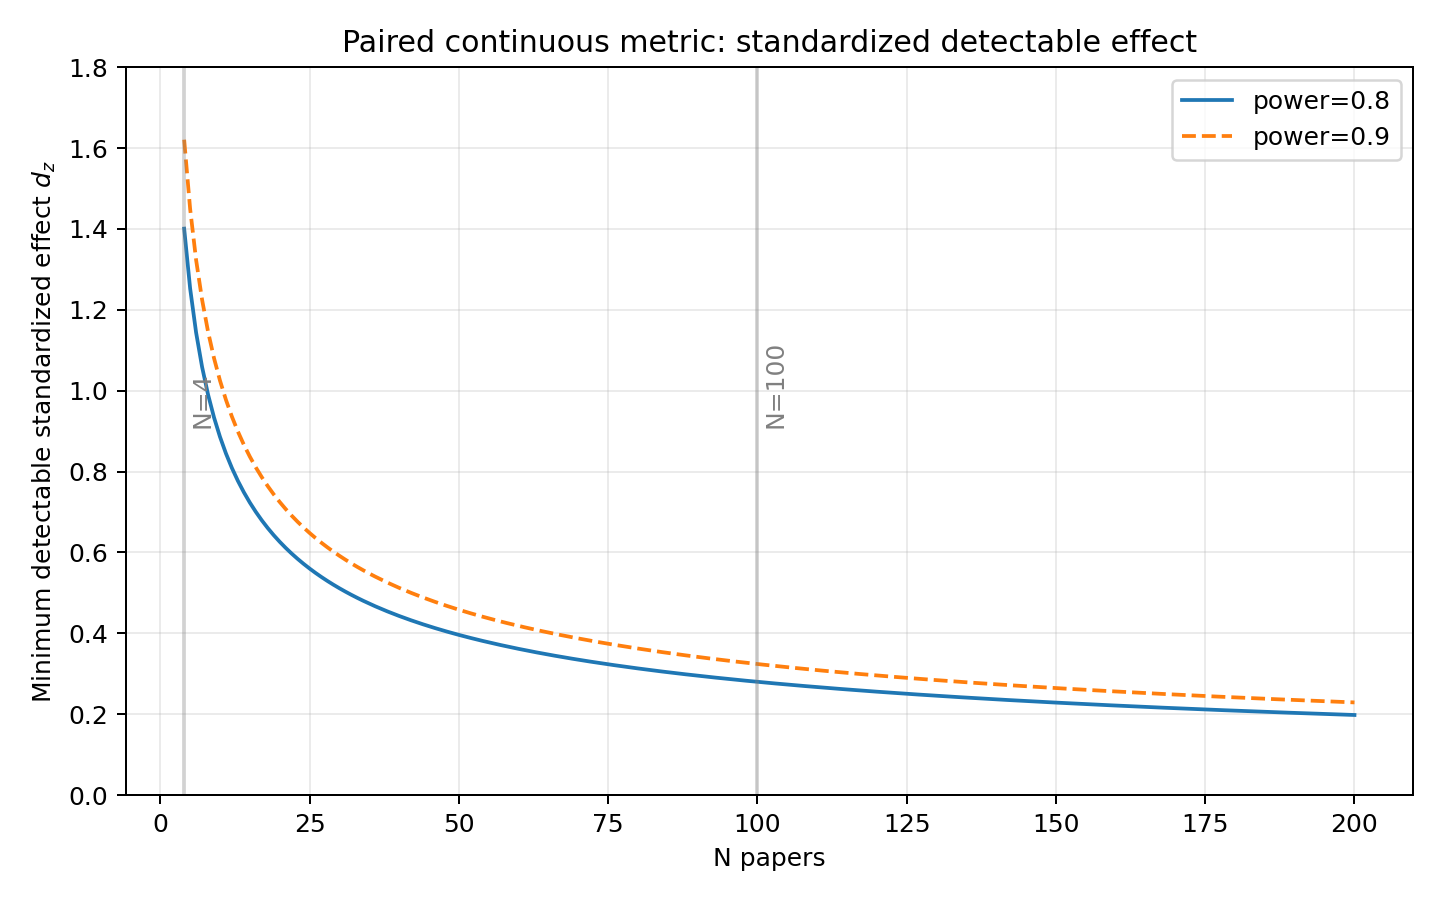
\includegraphics[width=0.86\linewidth]{figures/standardized_delta_vs_N.png}\caption{Paired continuous metric 的標準化 detectable effect。}\end{figure}
\begin{figure}[H]\centering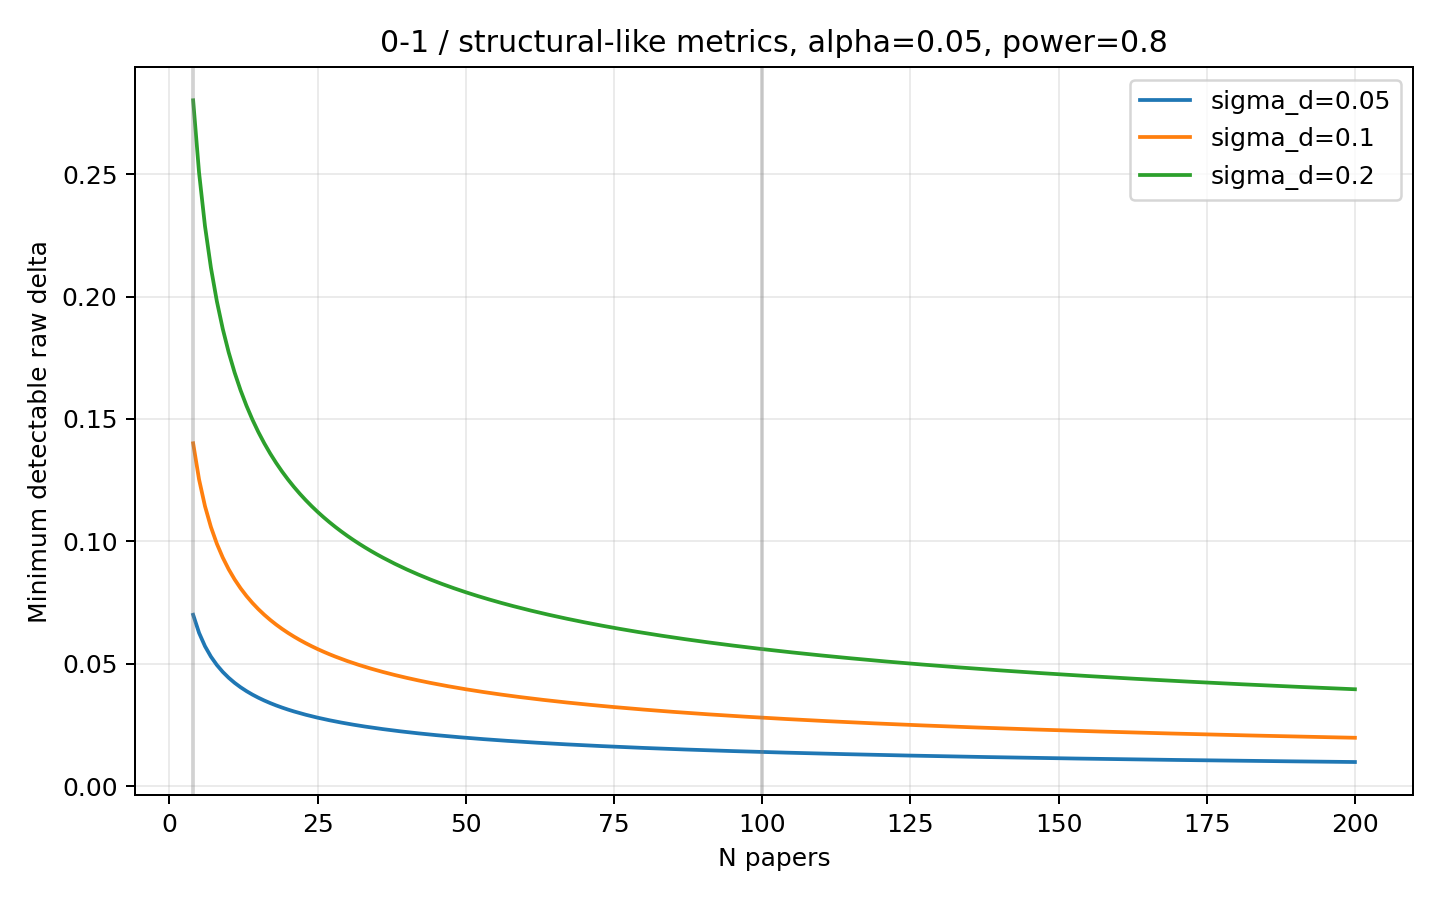
\includegraphics[width=0.86\linewidth]{figures/structural_raw_delta_vs_N.png}\caption{0--1 / Structural-like metric raw delta curve。}\end{figure}
\begin{figure}[H]\centering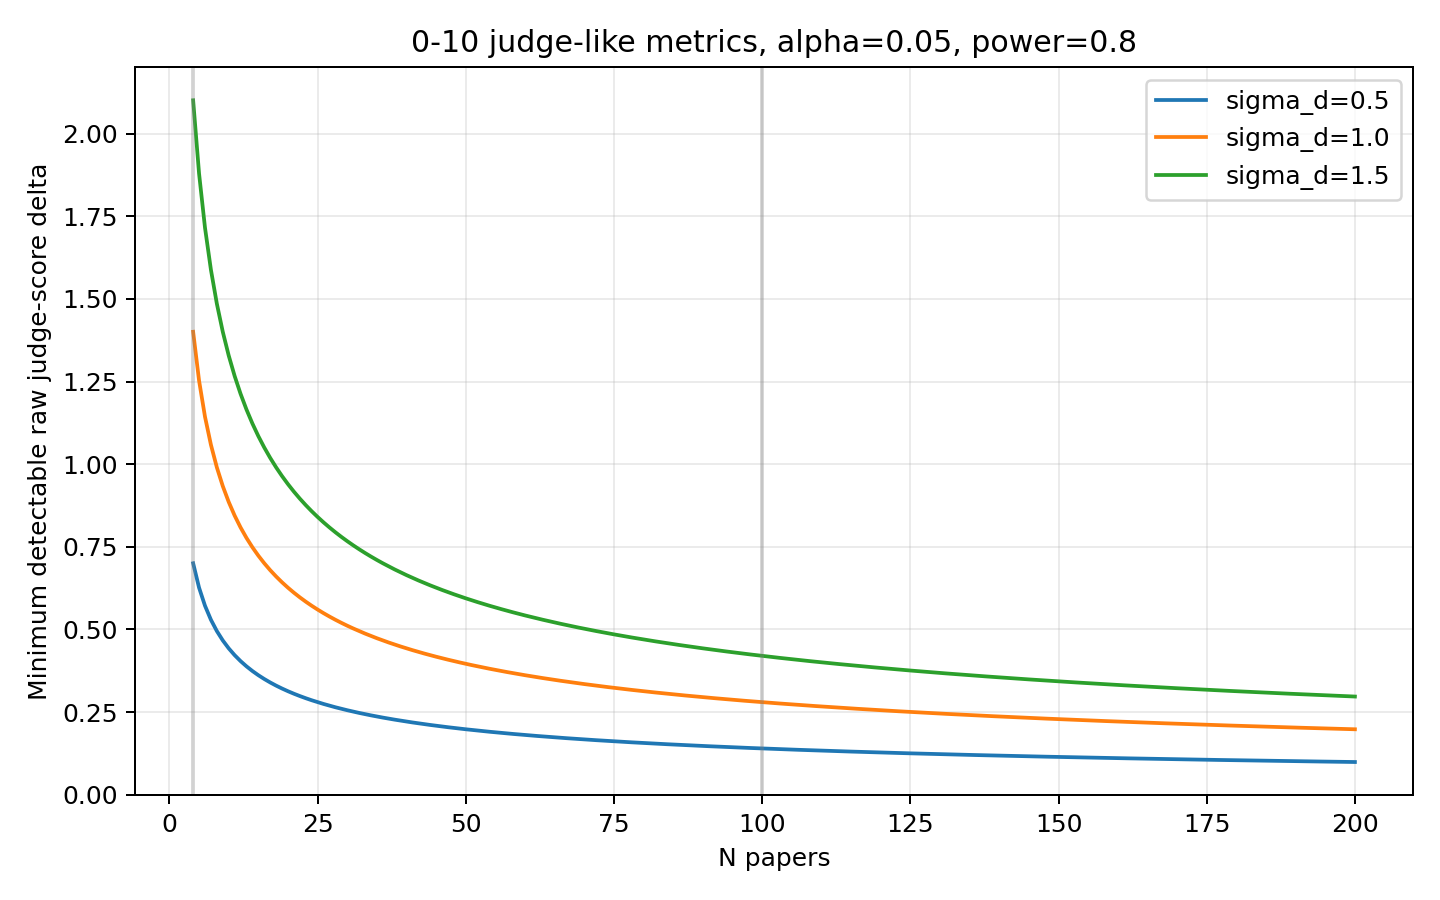
\includegraphics[width=0.86\linewidth]{figures/judge_raw_delta_vs_N.png}\caption{0--10 judge-like metric raw delta curve。}\end{figure}
\begin{figure}[H]\centering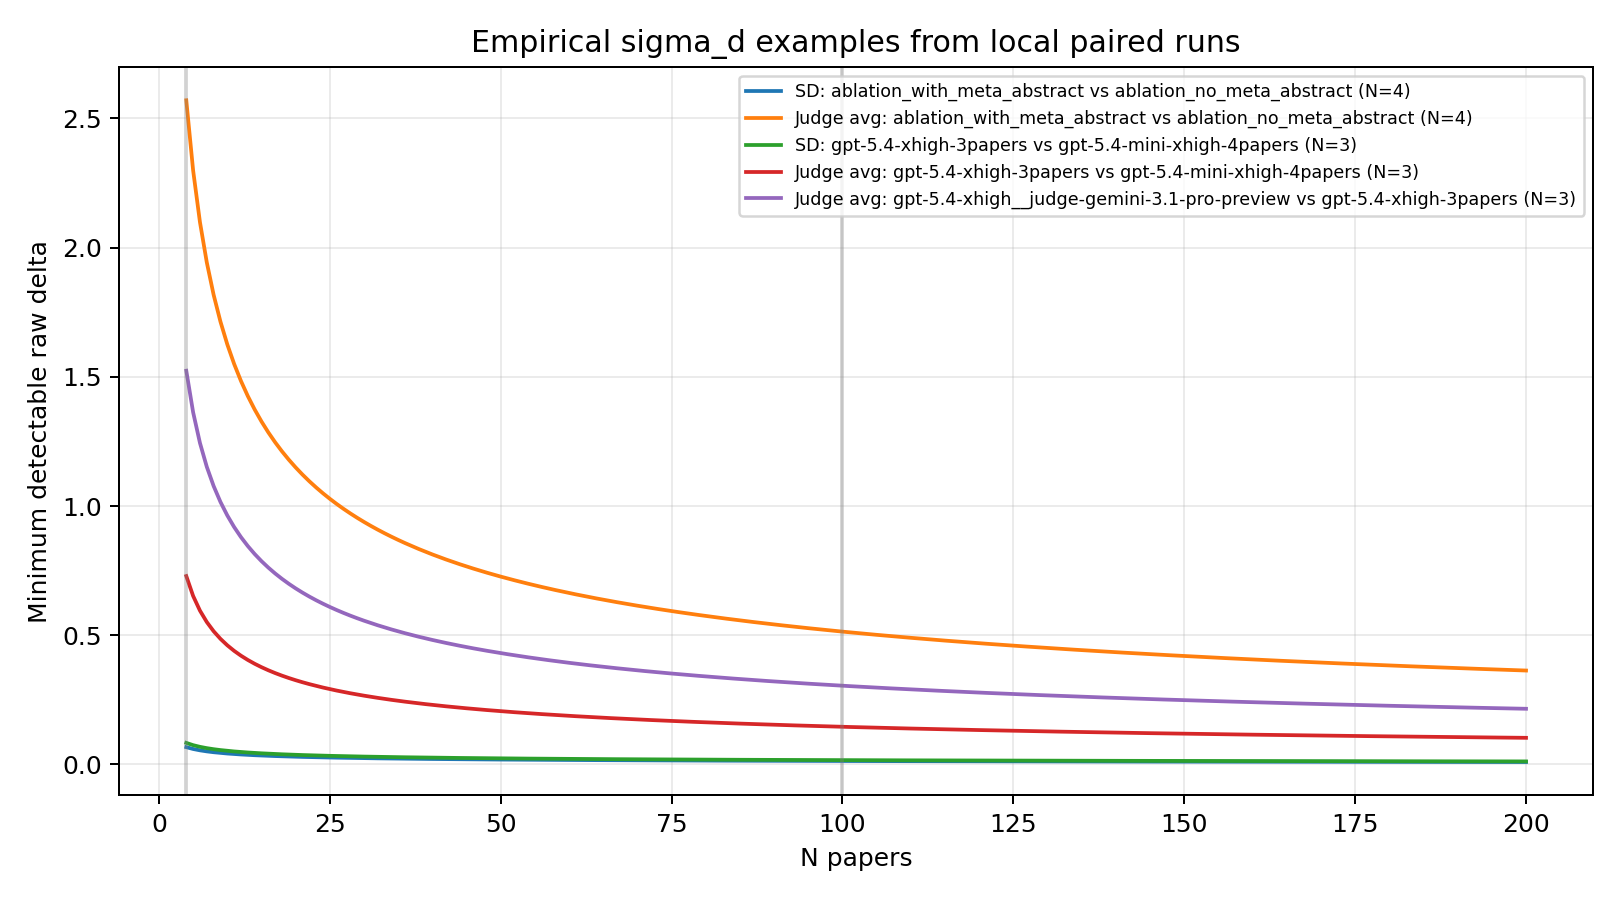
\includegraphics[width=0.86\linewidth]{figures/empirical_sigma_delta_vs_N.png}\caption{Local empirical paired sigma examples。}\end{figure}
\begin{figure}[H]\centering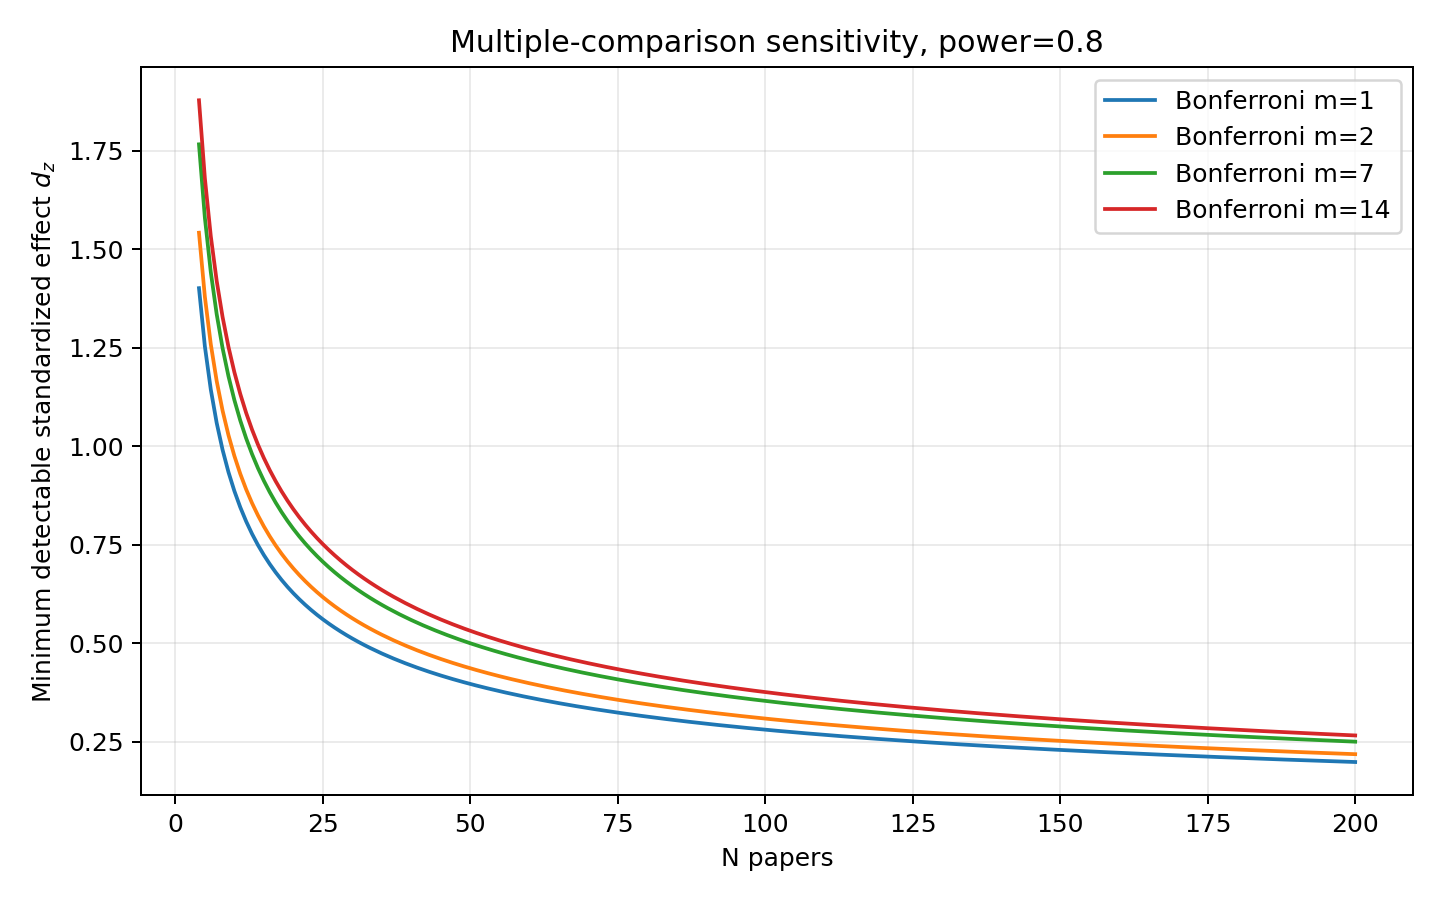
\includegraphics[width=0.86\linewidth]{figures/multiple_comparison_standardized_delta_vs_N.png}\caption{Bonferroni multiple-comparison sensitivity。}\end{figure}

\section*{Recommendations}
\begin{itemize}
\item N=4：只當 smoke。除非 raw gap 大到約 $1.4\sigma_d$，否則不應期待穩定顯著。
\item N=25：可檢出約 $0.56\sigma_d$，適合 early benchmark / ablation triage。
\item N=50：可檢出約 $0.40\sigma_d$，開始接近中等效果的正式比較。
\item N=100：可檢出約 $0.28\sigma_d$，適合主張 moderate but meaningful improvement。
\item 對 6D judge，不要把六維當成六個完全獨立樣本；若逐維報告，使用 Holm 或 Bonferroni，若作探索則用 BH/FDR。
\item 對 Structural Distance，先確定研究問題真的是 shape alignment；它不評語義、引用、標題品質。
\end{itemize}

\section*{Limitations}
本報告沒有重新跑 judge，也沒有把 auxiliary Reference reward 納入主曲線。Empirical sigma 只來自現有 local artifacts，且 N 很小，因此報告主體應視為 mathematical planning + source-confirmed metric inventory，而不是最終實驗結果。

\end{document}
